%%%%%%%%%%%%%%%%%%%%%%%%%%%%%%%%%%%%%%%%%%%%%%
%                insertmeeting
% 1) Title (something creative & funny?)
% 2) Date (MM/DD/YYYY)
% 3) Location (ex. Hagerty High School)
% 4) People/Committees Present 
% 5) Picture 
% 6) Start Time & Stop Time (ex. 12:30AM to 4:30PM)
%%%%%%%%%%%%%%%%%%%%%%%%%%%%%%%%%%%%%%%%%%%%%%
\insertmeeting 
	{Freight Frenzy Kick Off} 
	{09/18/21}
	{Hagerty High School}
	{Annika, Anouska, Clayton, Falon, Jensen, Nathan, Ritam, Rose, Samantha, Lilly}
	{Images/RobotPics/robot.jpg}
	{11:00 - 3:00}
	
\subsection*{General}
\noindent\hfil\rule{\textwidth}{.4pt}\hfil
\subsubsection*{Goals}
\begin{itemize}
    \item Successfully create a timeline and plan for the season on how we can succed 

\end{itemize} 

\noindent\hfil\rule{\textwidth}{.4pt}\hfil

\subsubsection*{Accomplishments}
We watched our reveal video for kickoff in the group projects room by the media center with our sister FTC team, 4227. We watched the video LIVE and came up with some questions for the game, solutions to the new problems and obstacles, etc.  we took a short lunch break eating some snacks, pizza, drinks. We headed up to the robotics room for a more team private discussion and talked about plans for the robot. We looked up ways that we could distinguish the blocks by weight since the weights are difficult to see, and are not visible in all 6 directions of the cube. We thought of different systems to distinguish cubes. An idea was to measure weights using a pulley to balance the game element. Another idea was to to use a spring to mark how far the weight would push the spring which we found to seem to be a more compact idea despite its many variables that could come with it. Another idea was using current to detect the weights to know whether it is heavy or light, and finally an idea that simply used a sensor that could indicate where the visible side of a cube has one or two weights to know if it is heavy or not. One idea we had initially was to use a pressure sensor, but the REV part was not allowed in FTC games. While we have many ideas for this, we will need to rule out which is best to use based on efficiency and how it will effect our design. We had different ideas for  coming up with a suitable drive train. The gap between the two poles of the raised barrier make it challenging to roll completely over it while it makes it complicated to decrease the width of our robot with a compact design. A suggestion was using custom wheels for the game. Ideally, pneumatic tires would be useful since they conform to the shape of the terrain. A design idea was using a material for wheels that would similarly be flexible on the terrain as pneumatic tires are such as rubber, foam, etc. we also thought about changing the shape of our tires to look less circular to climb over the barrier, but we would need a lot of testing for it to work well. For the Duck carousel, we simply wish to use a compliance wheel to spin the duck and set it to a power that is most efficient and test it with different positions of the duck placed on the carousel. One part that concerned me most with this game was the scoring for the supply hub. Since it rocks back and forth like a wobble goal, it is difficult to balance especially for if you were to place heavier game elements at the top. A lot of testing and understanding of the elements will be needed before we do much for strategizing. We need to know how the placement of our elements will effect the center of gravity of the supply hub. The intake and outake systems was discussed at large for our bot. An idea was that we create a robot that would use a lift mechanism traveling on a slope to the level of a platform on the alliance supply hub. While it was an interesting idea, it would be difficult to execute with the varying heights of the platforms. Another was an intake that would send game elements to the back of the bot and proceed to later lift it on a platform without turning too much. One of the issues we discussed with changing directions was the number of transitions the elements need to make that could cause mistakes and faults in our design. Despite all of this brainstorming and debates for the best types of designs and ideas that would be most efficient and effective on the robot, we continue to brainstorm and create ideas for new mechanisms since the release of the game. 
 

\begin{figure}[ht]
\centering
\begin{minipage}[b]{.50\textwidth}
  \centering
  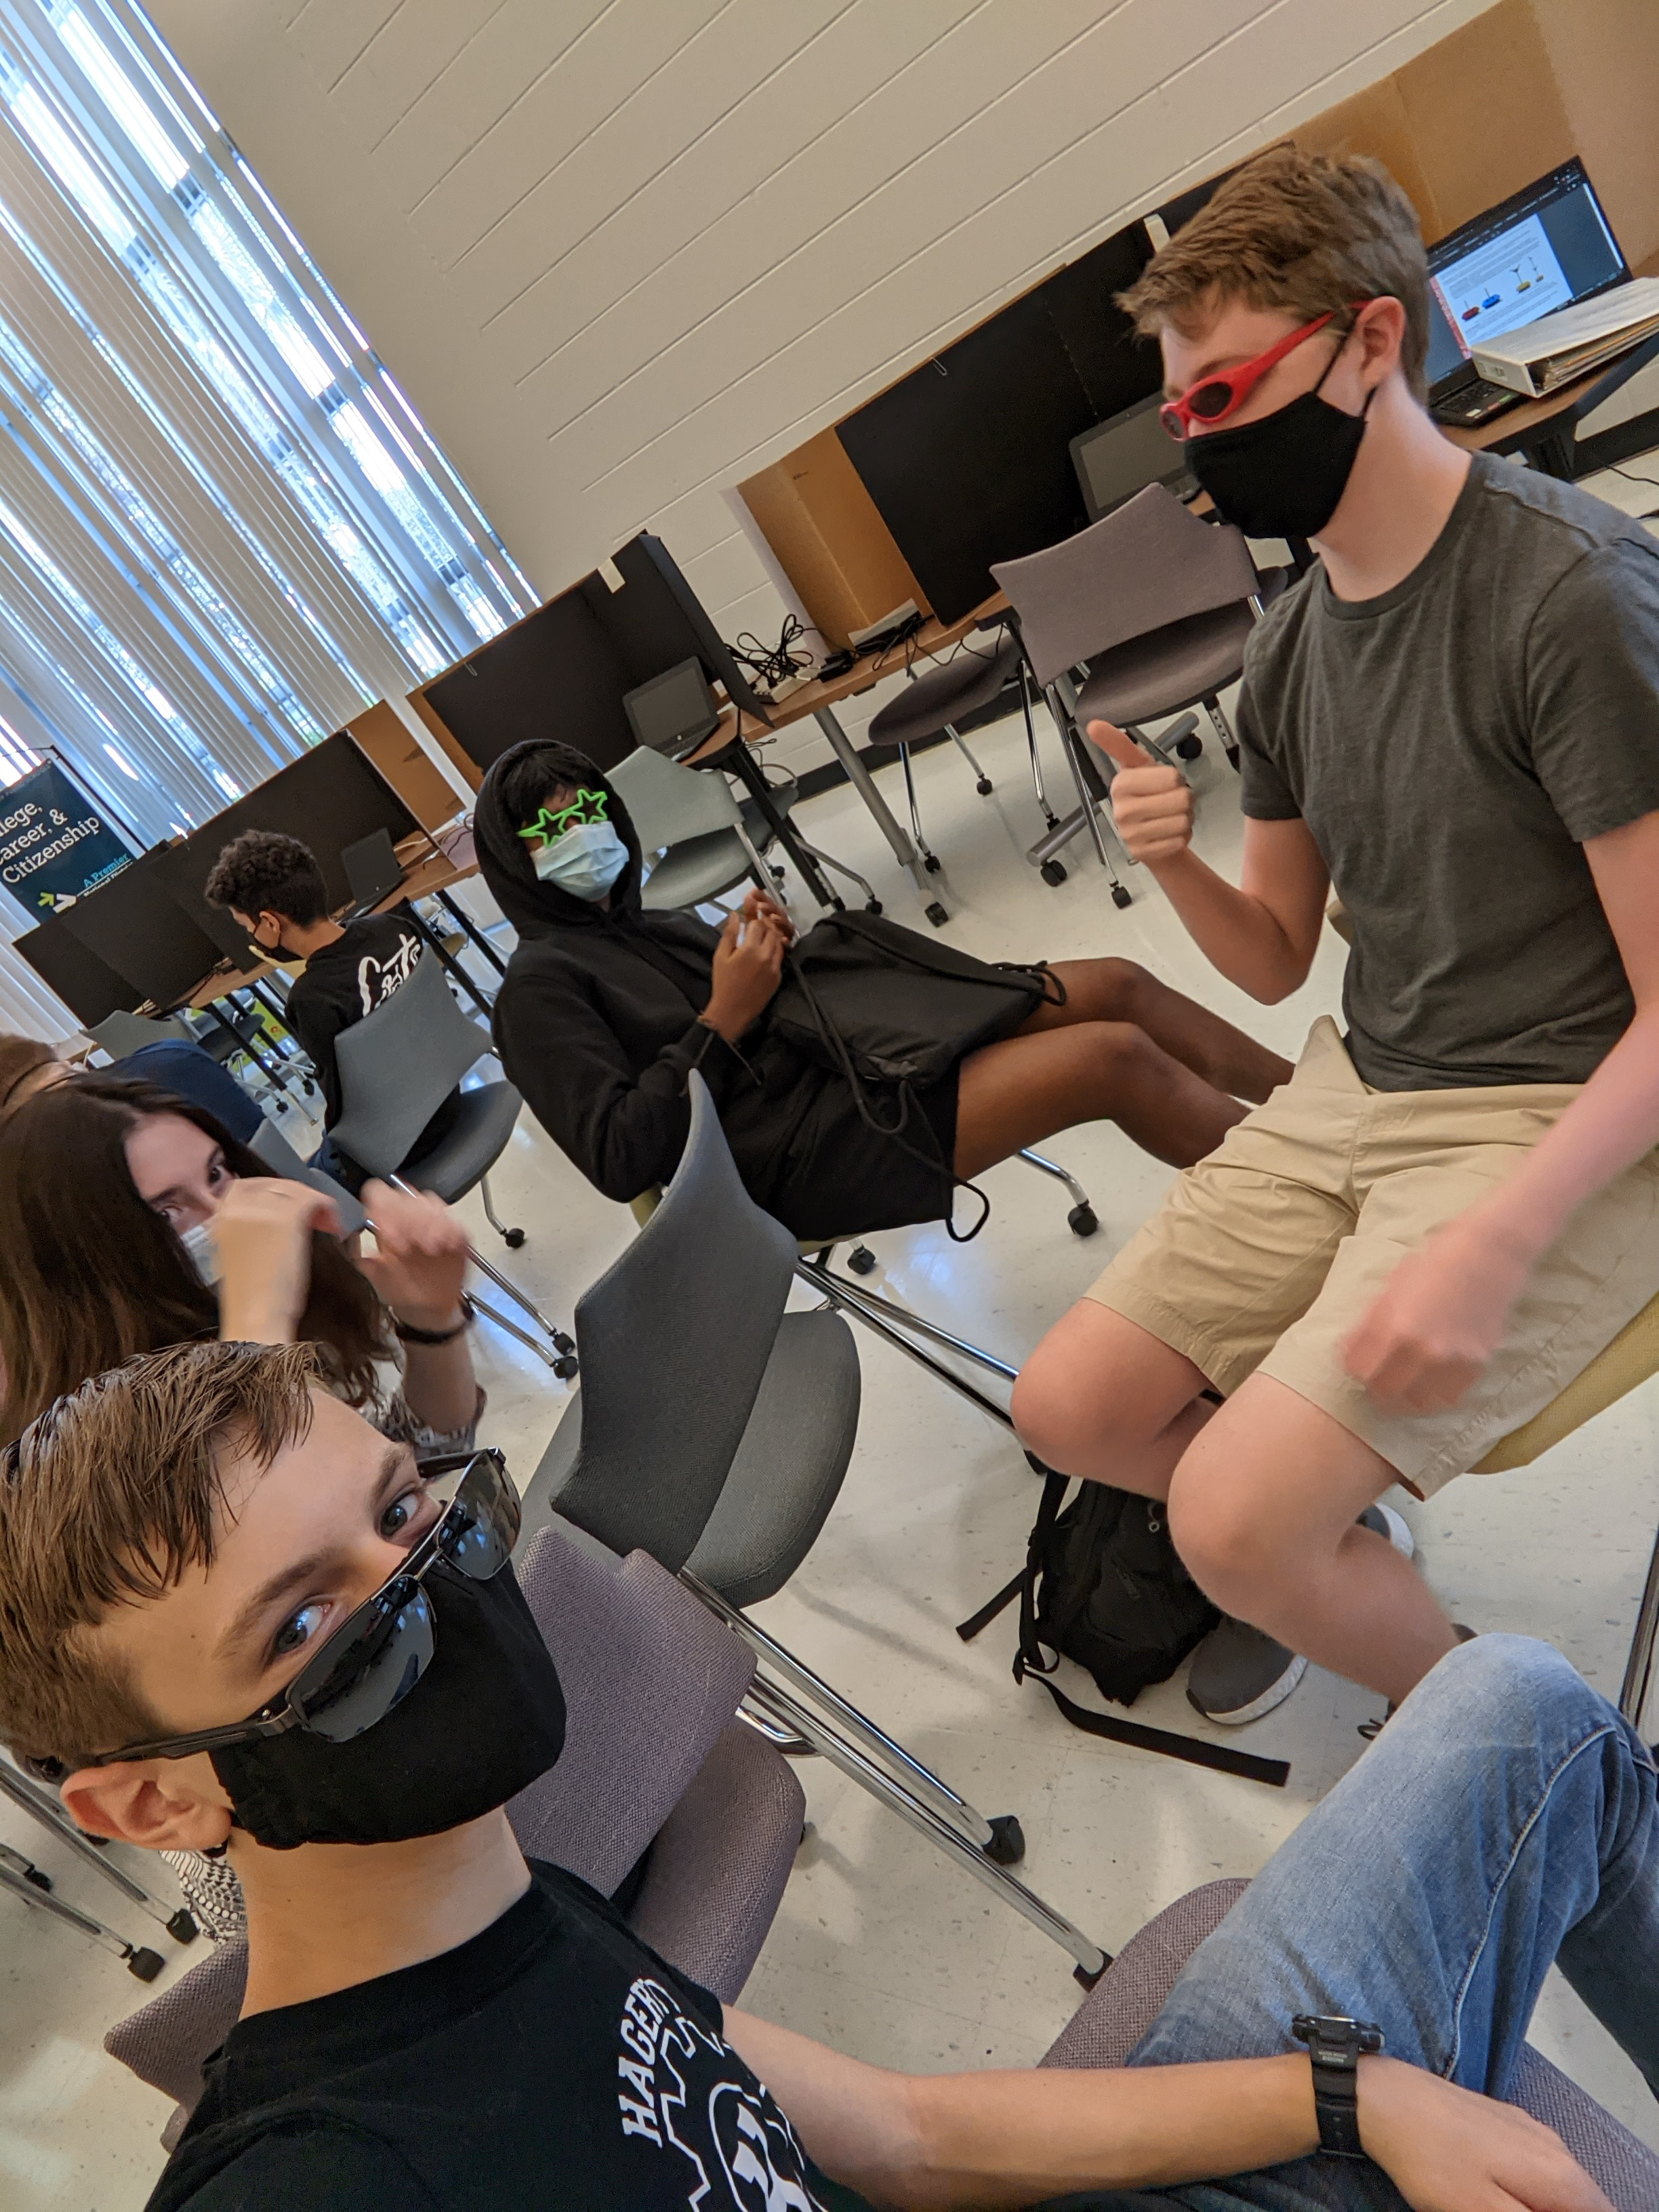
\includegraphics[width=0.8\textwidth]{Meetings/September/09-18-21/PXL_20210918_151448302 - Jensen Miller.jpg}
  \caption{4717 at Kickoff!}
  \label{fig:pic1}
\end{minipage}%
\hfill%
\begin{minipage}[b]{.50\textwidth}
  \centering
  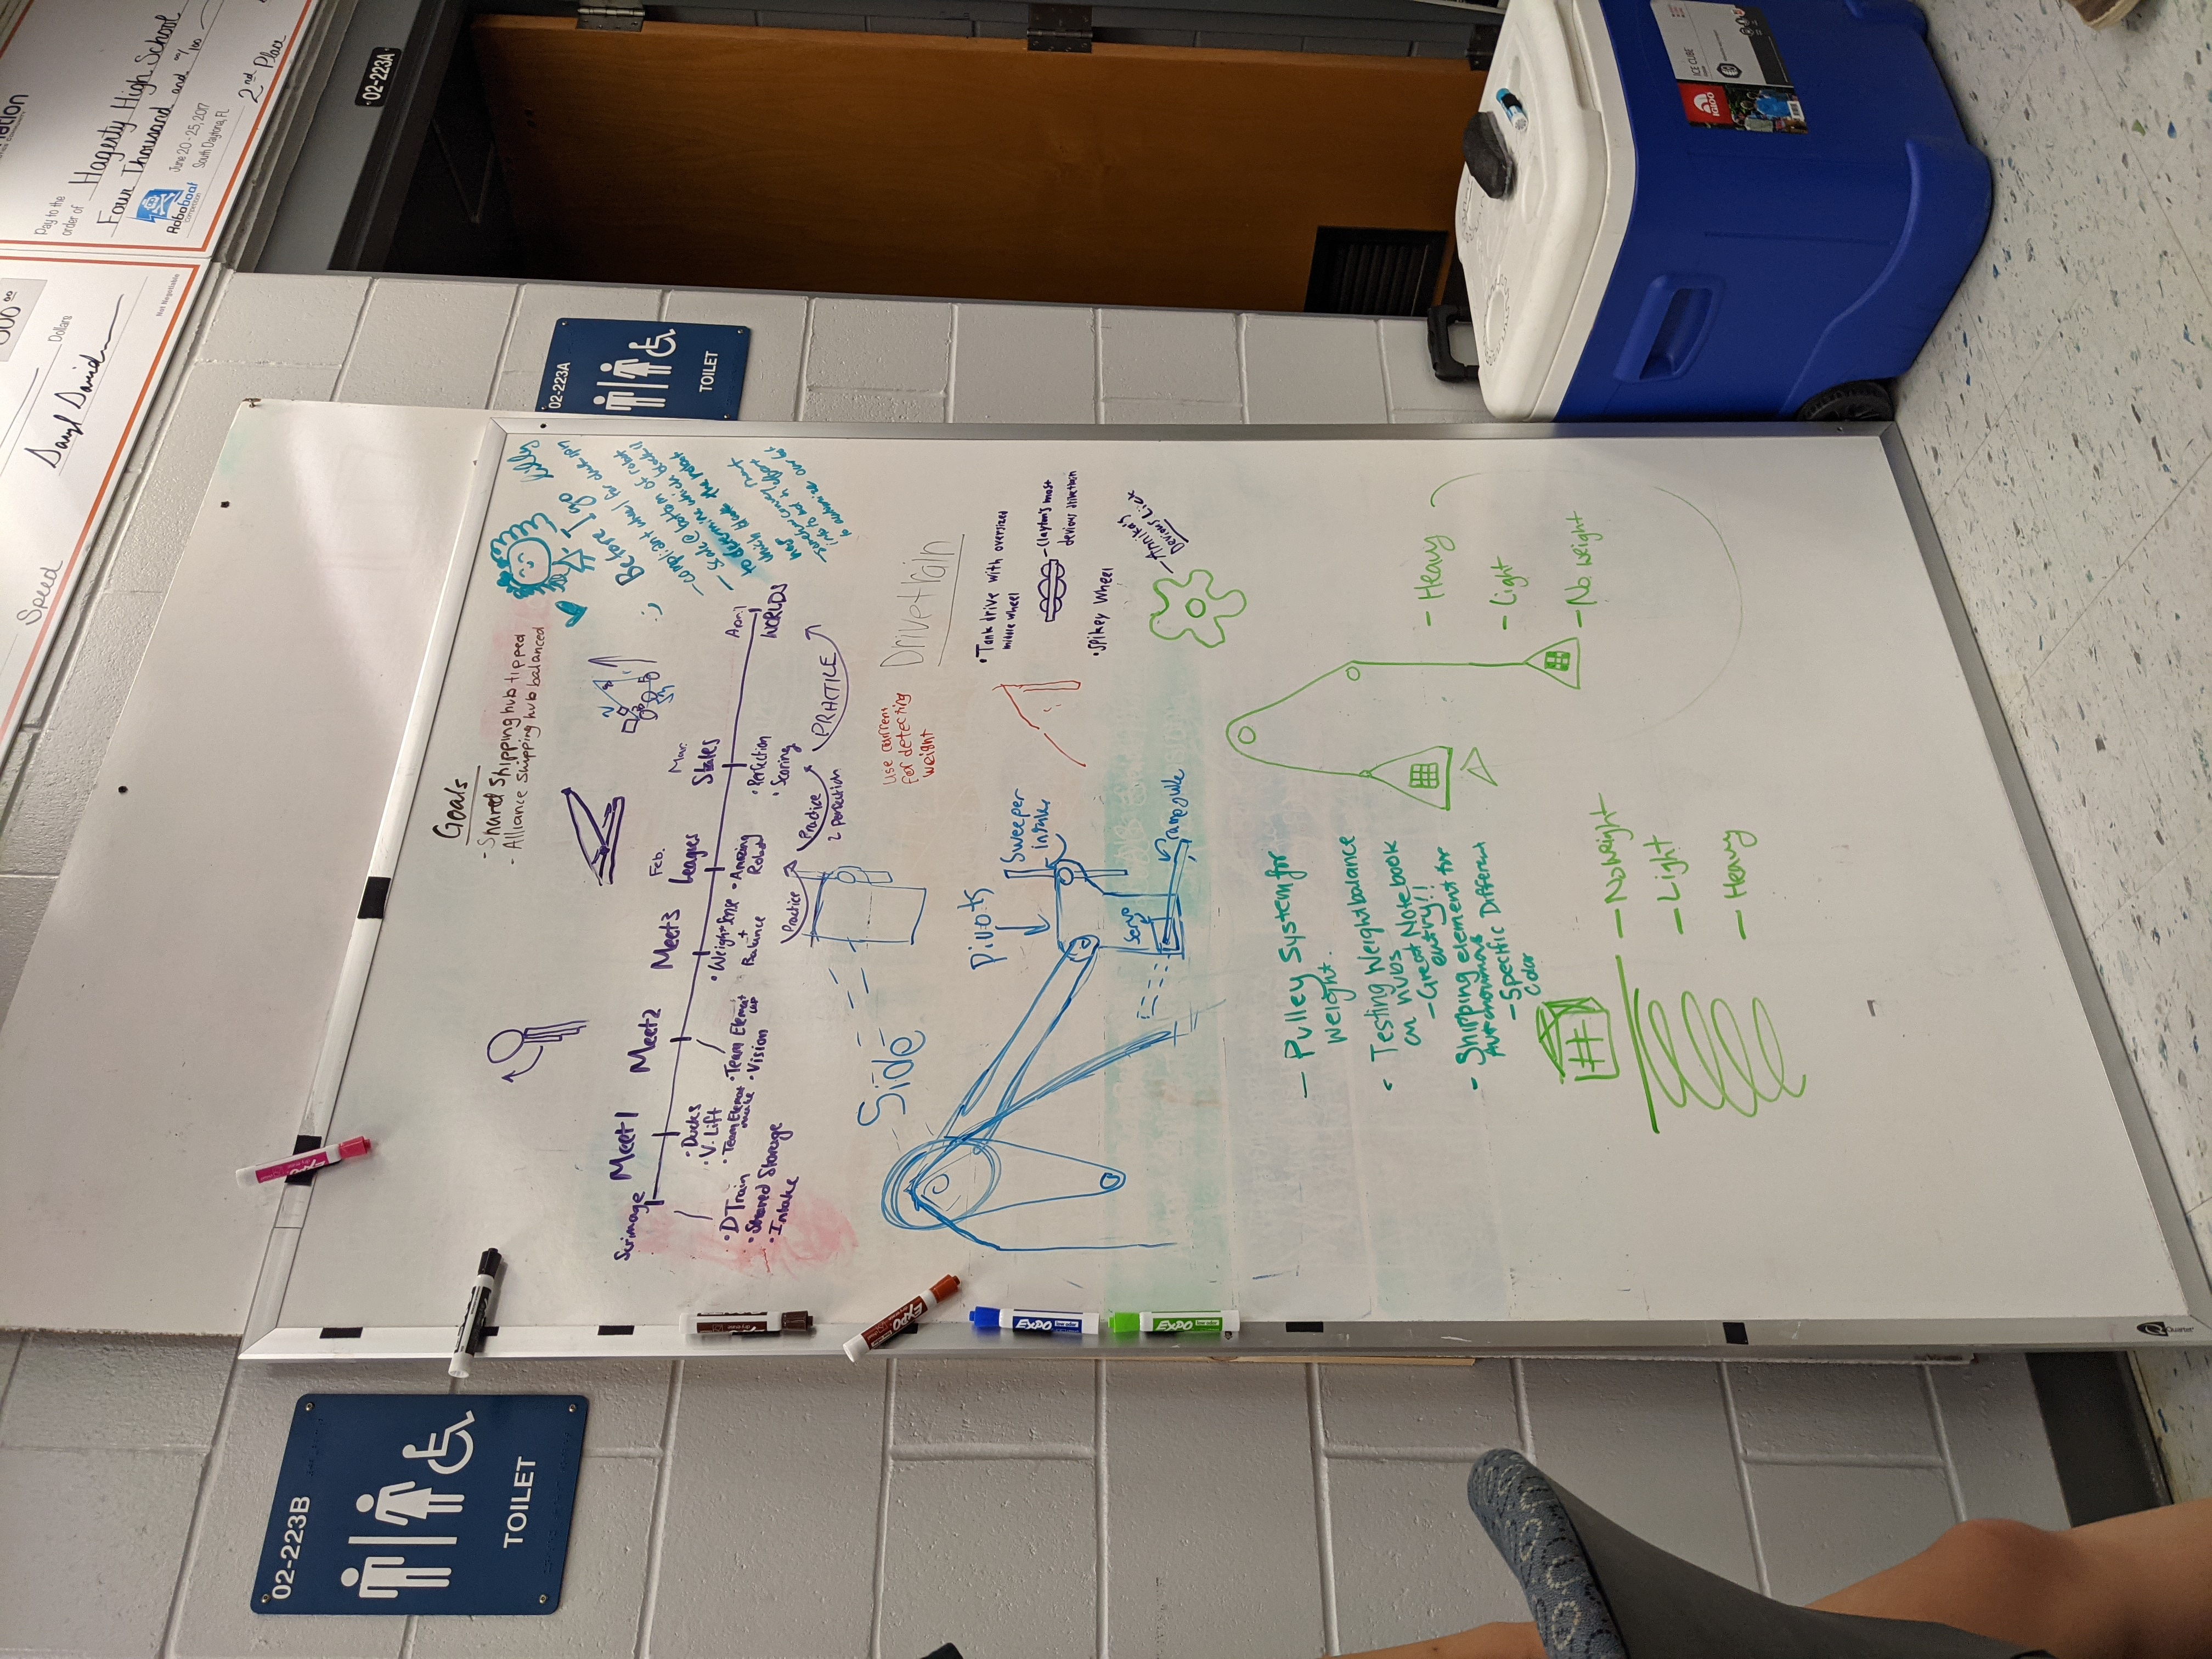
\includegraphics[width=0.8\textwidth]{Meetings/September/09-18-21/PXL_20210918_184637754 - Jensen Miller.jpg}
  \caption{Our brainstorming whiteboard for the next season.}
  \label{fig:pic2}
\end{minipage}
\end{figure}

\subsection*{Strategy}
\noindent\hfil\rule{\textwidth}{.4pt}\hfil
\subsubsection*{Goals}
\begin{itemize}
    \item Watch game reveal
		\item Come up with ideas for the season
		\item Brainstorm potential design ideas

\end{itemize} 

\noindent\hfil\rule{\textwidth}{.4pt}\hfil

\subsubsection*{Accomplishments}
In order to prepare our brains for out of the box thinking we started our meeting a bit before the game was revealed, we spent some time talking about what we thought the game would look like. In anticipation, we came up with several ideas of games we thought would be possible based on the name and logo of the game (image 1). As we were all eager to see the game and await the design challenges about to be presented, we had a lively discussion about all of our speculations and ideas for the season. Before we knew it, it was 12:00 and the game reveal was about to go live. Prepared with clipboards in hand, we were ready to start taking notes and making sketches of our initial design ideas.
The game reveal animation showed several different challenges for us to complete in the upcoming season (image 2). Starting out in the autonomous period, either a duck or shipping element is placed on 1 of 3 positions on the “barcode”. The robot can then place a preloaded freight onto the shipping hub and can earn bonus points for placing it on the level corresponding to where the duck or shipping element is on the barcode. Teams can also score points by delivering a duck from the carousel in the corner of the field. At the end of the autonomous period, there are two options for parking: one in the alliance’s storage unit (more points are awarded for being completely inside the square) and one in the warehouse(more points are awarded for being completely inside the warehouse).
In the tele-op period, the main objective is to move freight onto either the alliance shipping hub or the shared shipping hub. Points can be gained depending on what level of the alliance shipping hub freight is placed on. Teams can also be awarded points if the shared shipping hub is tipped towards their alliance’s direction. One thing we thought was notable about transporting freight is that each robot can only carry 1 piece of freight at any time. This will mean that efficient movement is key.
During the endgame period, teams can spin the carousel to deliver ducks onto the field. Teams are also allowed to place their team shopping element on top of their alliance shipping hub. At the very end of the match, points are earned for parking in the warehouse(more points are awarded for being completely inside the warehouse). Finally, extra points are awarded if a team’s alliance shipping hub is balanced and if the shared shipping hub is tilted in their direction.
While watching the video, we all made simple sketches and took notes about the game, so that afterwards we could discuss our thoughts and ideas (image 3 and 4). After talking about our initial thoughts, we moved on to a general strategy. It was clear that having a fast moving robot that can efficiently move cargo would be the key to success. This meant finding the most direct path between the warehouse and the alliance shipping hub in tele-op. We noticed that the gaps between the walls and the pvc pipe barriers around the cargo bay would be just big enough to fit a smaller robot through, meaning we could avoid slowly going over the barriers by going around them. Having a small robot will also help with the shared shipping hub, as there isn’t much room in the area. We also think that the carousel mechanism will also be an important part of the robot, especially in endgame. Another thing we took into consideration was ensuring that we had a unique design that would differentiate us from other robots. It is always important to us that we come up with entirely original designs and resist the common strategy of mimicking the most popular robot early on. This will prevent us from stagnating early in the season and will keep us innovating past our competition.
Moving on from strategy, we started discussing our plans for hardware. We used a white board in the room to draw out all of our ideas and to better convey what we were thinking to each other (image 5). Because we already built and tested a prototype intake, we all agreed that we should probably use the sweeper intake as it had worked the best while testing. Another aspect of hardware that we talked about was using a pass-through design, where the freight is picked up with an intake in the front, but the out take is on the back. This will prevent us from needing to turn around, saving precious time. Last year, we found that having several subsections of the robot (for example, an intake, lift, and shooter) that are seperate parts but that are meant to interact caused difficulty. Our problem came from the transference between the mechanisms, as we found that our rings would get stuck between two of the parts. Our plan for avoiding this problem is only having one mechanism, the intake, that acts as an intake, transference system, and out take. Using our intake prototype, we demonstrated this concept to get a better understanding of how it would actually function (image 6).  One of the other things that we discussed was differentiating between weights of the freight. Because there isn’t a weight sensor we can use, we thought about using a spring system that can only be compressed by the heavy freight. When the spring is compressed, a button connected to led lights would be pressed, which would indicate the weight of the blocks to the driveteam. We also talked about using a pulley system that would similarly uses the weight to mechanically move it up or down, indicating the weight (image 7). Knowing the different weights of freight would help us decide where to place it. Placing heavier freight on the shared shipping hub would allow us to tip it in our direction easier and with less pieces of freight. 
One of the last things we talked about was the drive train. Because of the pipes blocking off the warehouse, we will need to make a drivetrain that can easily go over bumps without getting stuck. Unfortunately, our mecanum drivetrain will probably not work this season because the rollers on the wheels will slip on the pipes, making the robot unable to get over them. We might be able to design a tank drive similar to what we have built in past years, but we would need to change the plates to make them farther off the ground, and we have a suspicion that the middle drop center wheel will get stuck in between the barriers. Because the drivetrain is going to be one of the most difficult parts to design, we were unable to come up with a final plan for the drivetrain during this meeting. It is still a high priority because we need a drivetrain before we can build any other parts of the robot.
Finally, we made a timeline for ourselves planning out where we want to be at each major landmark in the season. (image 8) Because we faced problems with our time management last year, we know that we have to stay on top of our goals this year.
The whole team is very excited about the game and we are all ready to start building and programming. Because the drivetrains we know well might not function with this year’s game building prototypes is going to be very important. Building these prototypes is integral so we can move onto the next stages of our design and stay on track with our timeline.





